\section{球密度による高速化への影響}
\label{sec:density}
超音波照射された擬塑性流体中を落下する球における高速化に関して,球密度による影響を考えるため,落下球の密度を変化させて実験を行った.実験条件をTable\ref{table:exp-conditions}に示す.落下球の高速化に関して,式(\ref{eq:Udiff})より球径による影響を受けるが,今回の実験条件において密度変化による影響よりも十分に小さいものとして,球径は同一として考える.

超音波照射された擬塑性流体中に,密度を変化させ球を落下させた結果をFig.\ref{fig:0.05-0.2}-\ref{fig:1.5}に示す.この結果より,超音波照射されていない状態の終端速度を求めた結果をFig.\ref{fig:rhoUT}に示す.縦軸は終端速度$U_\text{T}$,横軸は密度差$\Delta\rho$である.密度差が大きくなると,終端速度が大きくなった.超音波照射されていない落下球の理論式(\ref{eq:UT})より,落下球と溶液の密度差のみをパラメータとして考えると終端速度は次式で表される.
\begin{eqnarray}
    U_\text{off}\sim \left(\Delta\rho\right)^{\frac{1}{n}} .
    \label{eq:UT_rho}
\end{eqnarray}
式(\ref{eq:UT_rho})を用いて,超音波照射されていない落下球の終端速度を整理した結果をFig.\ref{fig:rhoUT_n}に示す.縦軸は終端速度$U_\text{off}$,横軸は密度差のみによる影響を考慮した$\left(\Delta\rho\right)^{\left(1/n\right)}$である.本実験において,$0.17\leqq n\leqq0.59$であり,式(\ref{eq:UT_rho})において密度差の指数部は$1.69<1/n<5.89$となる.ゆえに密度差$\Delta\rho$が増加すると終端速度$U_\text{off}$も増加したと考えられる.

また,濃度ごとに高速化度合いを求めた結果をFig.\ref{fig:rhoUdiff}に示す.縦軸は高速化度合$U_\text{on}/U_\text{off}$,横軸は密度差$\Delta\rho$である.PAA濃度0.2,1.5wt.\%においてはあまり高速化が見られなかった.PAA濃度0.5,0.7wt.\%において,密度差が大きくなると高速化が顕著にみられた.一方で,PAA濃度1.0wt.\%においては,密度差が大きくなると高速化が顕著にみられた.PAA濃度1.3wt.\%においては,全体的に高速化がみられ,密度差による影響があまり顕著にみられない.

超音波照射された擬塑性流体中を落下する球の高速化に対する,落下球の密度による影響を考える.\ref{sec:UTdiff}節にて示した,超音波照射された落下球の終端速度の理論式(\ref{eq:U_ABL})と超音波されていない落下球の終端速度の理論式(\ref{eq:UT})より,
\begin{eqnarray}
    \frac{U_\text{on}}{U_\text{off}} \sim \left(\frac{\Delta\rho{}g}{3}\right)^{\frac{n-1}{n}}\cdot\frac{2-n}{n}\cdot\frac{\delta}{\mu_{ABL}}\cdot\left(\frac{k}{a}\right)^{\frac{1}{n}} ,
    \label{eq:UdiffRho}
\end{eqnarray}
となる.本実験において,落下球と溶液の密度差のみをパラメータとして考えるため,超音波照射に伴う高速化は式(\ref{eq:UdiffRho})より次式で表される.
\begin{eqnarray}
    \frac{U_\text{on}}{U_\text{off}} \sim \left(\Delta\rho{}\right)^{\frac{n-1}{n}} .
    \label{eq:UdiffRho2}
\end{eqnarray}
式(\ref{eq:UdiffRho2})を用いて,落下球と流体の密度差と超音波照射による高速化度合いを整理した結果をFig.\ref{fig:rhoUdiff_n}に示す.縦軸は高速化度合い$U_\text{on}/U_\text{off}$,横軸は密度差のみによる影響を考慮した$\Delta\rho^{\left(\left(n-1\right)/n\right)}$である.本実験において,式(\ref{eq:UdiffRho2})の指数部は$-4.9<(n-1)/n<-0.69$となり,密度差$\Delta\rho$が増加すると高速化度合い$U_\text{on}/U_\text{off}$は減少する.PAA濃度0.2wt\%において,あまり高速化が見られず密度差による影響が見られなかった.PAA濃度0.5,0.7wt.\%において,密度差が大きくなると高速化が顕著にみられ,式(\ref{eq:UdiffRho2})の理論通りとなった.一方で,PAA濃度1.0wt.\%においては,理論式とは異なり,密度差が大きくなると高速化が顕著にみられた.これは密度差以外の要因によるものだと考えられる.同様に,PAA濃度1.3wt.\%においては,全体的に高速化がみられ,密度差以外による影響が大きいと考えられる.以上より,超音波照射による高速化に対して,密度差による影響が存在するが,高速化が見られる低濃度域(0.5,0.7wt.\%)のみに顕著にみられ,それ以上の濃度では密度差以外による要因が大きく影響を与えていると考えられる.

\begin{figure}[ht]
    \centering
    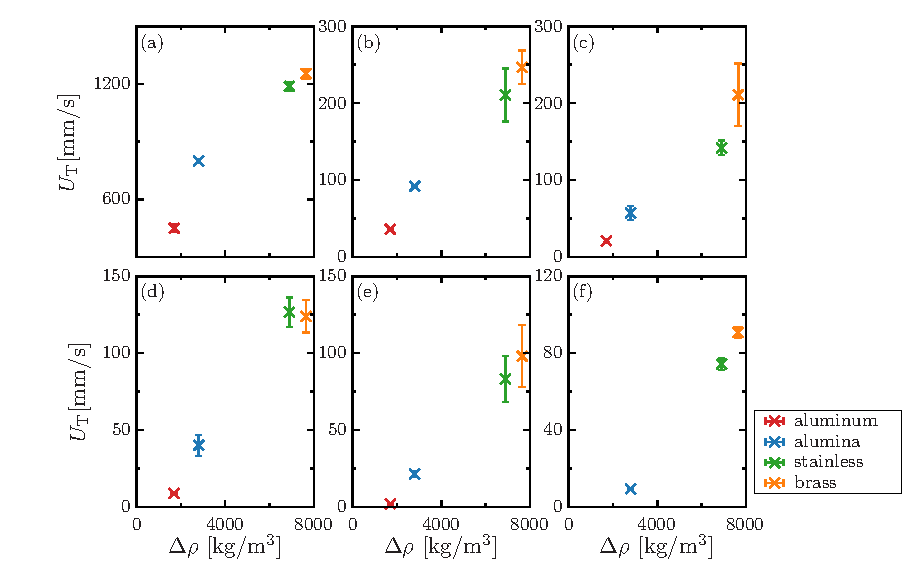
\includegraphics[width=1.0\textwidth]{./5-Results/rhoUT.eps}
    \caption{Termination velocity by density difference in PAA solution (a)0.2wt.\%, (b)0.5wt.\%, (c)0.7wt.\%, (d)1.0wt.\%, (e)1.3wt.\%, (f)1.5wt.\%.}
    \label{fig:rhoUT}
\end{figure}

\begin{figure}[ht]
    \centering
    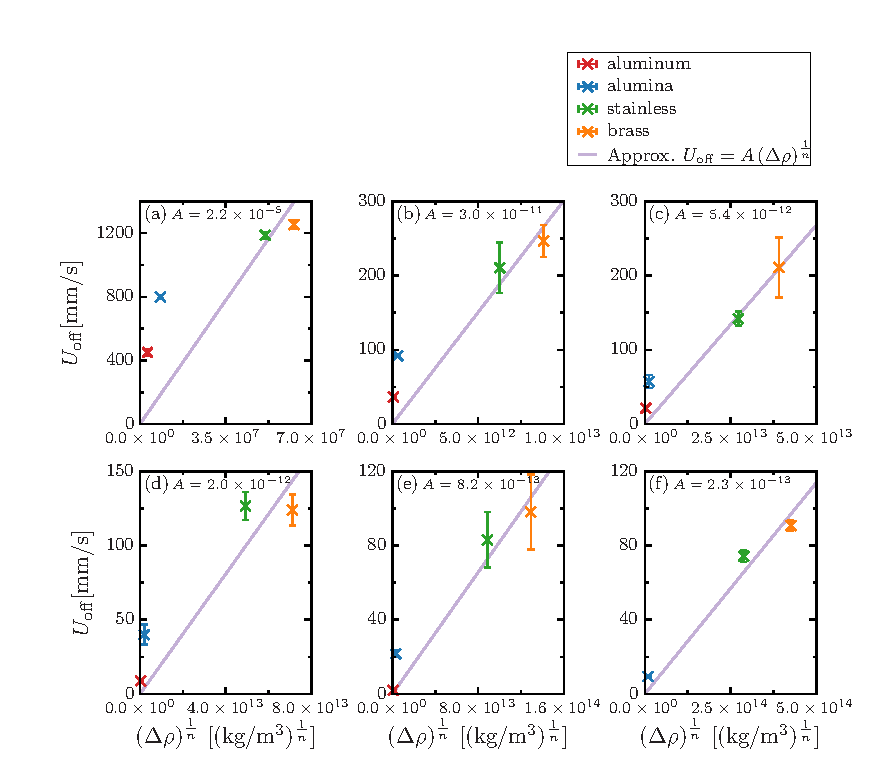
\includegraphics[width=1.0\textwidth]{./5-Results/rhoUT_index_n.eps}
    \caption{Termination velocity by density difference by index $n$ in PAA solution (a)0.2wt.\%, (b)0.5wt.\%, (c)0.7wt.\%, (d)1.0wt.\%, (e)1.3wt.\%, (f)1.5wt.\%.}
    \label{fig:rhoUT_n}
\end{figure}

\begin{figure}[ht]
    \centering
    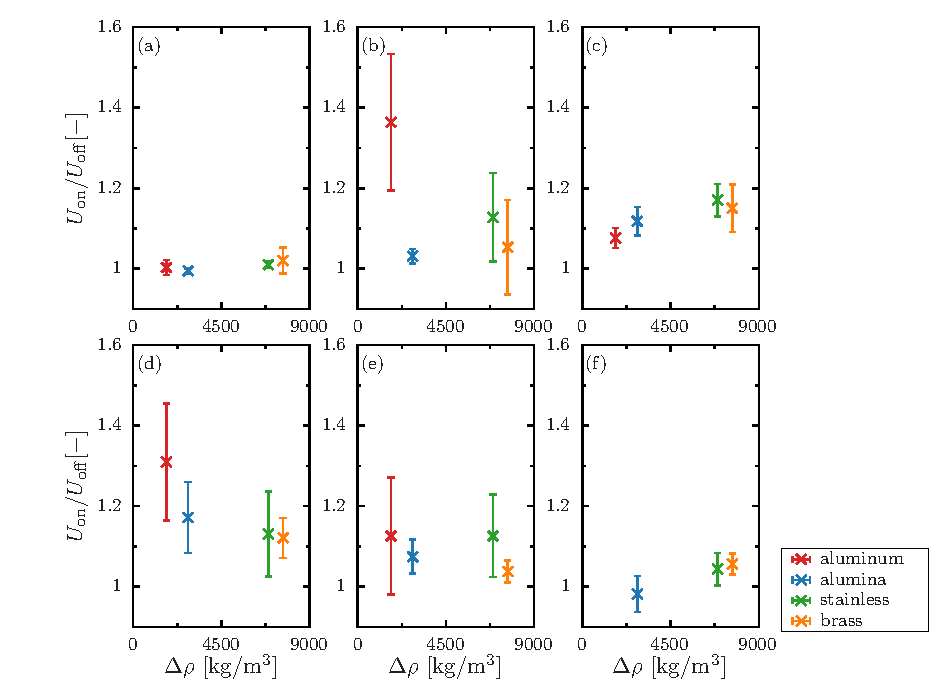
\includegraphics[width=1.0\textwidth]{./5-Results/rhoUdiff.eps}
    \caption{Velocity ratio versus density difference in PAA solution (a)0.2wt.\%, (b)0.5wt.\%, (c)0.7wt.\%, (d)1.0wt.\%, (e)1.3wt.\%, (f)1.5wt.\%.}
    \label{fig:rhoUdiff}
\end{figure}

\begin{figure}[ht]
    \centering
    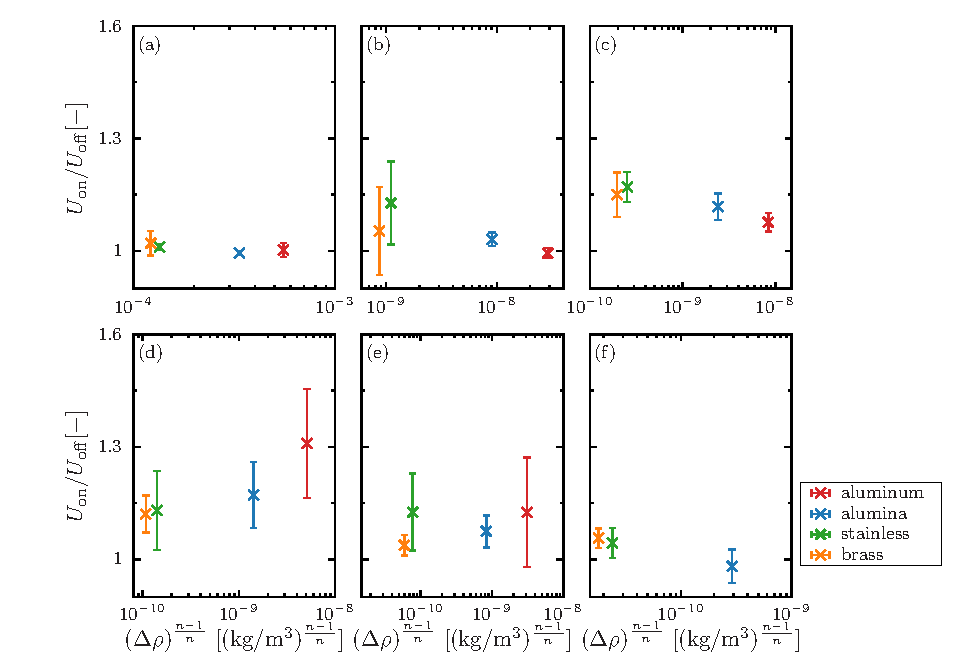
\includegraphics[width=1.0\textwidth]{./5-Results/rhoUdiff_index_n.eps}
    \caption{Velocity ratio versus density difference by index $n$ in PAA solution (a)0.2wt.\%, (b)0.5wt.\%, (c)0.7wt.\%, (d)1.0wt.\%, (e)1.3wt.\%, (f)1.5wt.\%.}
    \label{fig:rhoUdiff_n}
\end{figure}
